% -*- mode: LaTeX; TeX-PDF-mode: t; -*- # Tell emacs the file type (for syntax)
% LaTeX path to the root directory of the current project, from the directory in which this file resides
% and path to econtexPaths which defines the rest of the paths like \FigDir
\providecommand{\econtexRoot}{}\renewcommand{\econtexRoot}{.}
\providecommand{\econtexPaths}{}\renewcommand{\econtexPaths}{\econtexRoot/Resources/econtexPaths}
% -*- mode: LaTeX; TeX-PDF-mode: t; -*- 
% The \commands below are required to allow sharing of the same base code via Github between TeXLive on a local machine and Overleaf (which is a proxy for "a standard distribution of LaTeX").  This is an ugly solution to the requirement that custom LaTeX packages be accessible, and that Overleaf prohibits symbolic links
\providecommand{\packages}{\econtexRoot/Resources/texmf-local/tex/latex}
\providecommand{\econtex}{\packages/econtex}
\providecommand{\econark}{\econtexRoot/Resources/texmf-local/tex/latex/econark}
\providecommand{\econtexSetup}{\econtexRoot/Resources/texmf-local/tex/latex/econtexSetup}
\providecommand{\econtexShortcuts}{\econtexRoot/Resources/texmf-local/tex/latex/econtexShortcuts}
\providecommand{\econtexBibMake}{\econtexRoot/Resources/texmf-local/tex/latex/econtexBibMake}
\providecommand{\econtexBibStyle}{\econtexRoot/Resources/texmf-local/bibtex/bst/econtex}
\providecommand{\econtexBib}{economics}
\providecommand{\notes}{\econtexRoot/Resources/texmf-local/tex/latex/handout}
\providecommand{\handoutSetup}{\econtexRoot/Resources/texmf-local/tex/latex/handoutSetup}
\providecommand{\handoutShortcuts}{\econtexRoot/Resources/texmf-local/tex/latex/handoutShortcuts}
\providecommand{\handoutBibMake}{\econtexRoot/Resources/texmf-local/tex/latex/handoutBibMake}
\providecommand{\handoutBibStyle}{\econtexRoot/Resources/texmf-local/bibtex/bst/handout}

\providecommand{\FigDir}{\econtexRoot/Figures}
\providecommand{\CodeDir}{\econtexRoot/Code}
\providecommand{\DataDir}{\econtexRoot/Data}
\providecommand{\SlideDir}{\econtexRoot/Slides}
\providecommand{\TableDir}{\econtexRoot/Tables}
\providecommand{\ApndxDir}{\econtexRoot/Appendices}

\providecommand{\ResourcesDir}{\econtexRoot/Resources}
\providecommand{\rootFromOut}{..} % APFach back to root directory from output-directory
\providecommand{\LaTeXGenerated}{\econtexRoot/LaTeX} % Put generated files in subdirectory
\providecommand{\econtexPaths}{\econtexRoot/Resources/econtexPaths}
\providecommand{\LaTeXInputs}{\econtexRoot/Resources/LaTeXInputs}
\providecommand{\LtxDir}{LaTeX/}
\providecommand{\EqDir}{\econtexRoot/Equations} % Put generated files in subdirectory

\providecommand{\local}{\LaTeXInputs/local}

\documentclass{beamer}
\usepackage{import}
\usepackage{ulem}
\usepackage[Overlays]{optional}
\usepackage{ifthen}
\usepackage{\econtexShortcuts}
%\usepackage{bbm}
\providecommand{\Ex}{\ensuremath{\mathbb{E}}} % Expectations operator defined in econtex.cls
\usepackage{\LaTeXInputs/SolvingMicroDSOPs}
\usepackage{econark}
% if this is uncommented, bullets are shown step by step; comment out to make printable version
\beamerdefaultoverlayspecification{<+->}

% MPCMatch
\provideboolean{MPCMatchVersion}
\setboolean{MPCMatchVersion}{true}
\setboolean{MPCMatchVersion}{false}
\newcommand{\MPCMatch}{\ifthenelse{\boolean{MPCMatchVersion}}}

\newboolean{DiscountSubOn}
\setboolean{DiscountSubOn}{false}
\providecommand{\TimeFactor}{\Discount}
\ifthenelse{\boolean{DiscountSubOn}}{\Discount_{t+1}}{}
\newcommand{\ifTimeSubT}{}
\ifthenelse{\boolean{DiscountSubOn}}{\renewcommand{\ifTimeSubT}{_{T}}}{}
\newcommand{\ifTimeSubNext}{}
\ifthenelse{\boolean{DiscountSubOn}}{\renewcommand{\ifTimeSubNext}{_{t+1}}}{}

\newboolean{RfreeSubOn}
\setboolean{RfreeSubOn}{false}
\providecommand{\R}{\Rfree}
\ifthenelse{\boolean{RfreeSubOn}}{\Rfree_{t+1}}{}

\usepackage{ifthen}
\newboolean{WithOverlays}
\setboolean{WithOverlays}{true}
\usepackage{optional}
\opt{NoOverlays}{\setboolean{WithOverlays}{false}\beamerdefaultoverlayspecification{}}
\usepackage{moreverb}

\usepackage{cancel}
\usepackage{econtexShortcuts}
\usepackage{wasysym}
%\usepackage{dcolumn}
% \usepackage[notocbib]{apacite}
%\renewcommand{\frametitle}{\textbf\frametitle}


% Jirka's definitions
\usepackage[authoryear]{natbib}
\definecolor{jirkasred}{rgb}{0.9,0,0}
\newcommand{\jemph}[1]{{\color{jirkasred}#1}}
\def\newblock{\hskip .11em plus .33em minus .07em}

\mode<presentation>
{
  \usetheme{default}
  % or ...
  \setbeamercovered{transparent}
}

% if this is on, bullets are shown step by step
% \beamerdefaultoverlayspecification{<+->}

%\setbeamertemplate{navigation symbols}{}  % Take away navigation symbols

\usetheme{Frankfurt}

%_____________ Opening slide _______________________

\begin{document}

%\begin{verbatimwrite}{./SolvingMicroDSOPs-Slides-body.tex}

\title[SolvingMicroDSOPs]{\textbf{Structural Estimation of Dynamic Stochastic\\ Optimizing Models of Intertemporal Choice \\ \LARGE{For Dummies!}}}
\author[Carroll]{Christopher Carroll\inst{1}}

\institute{
  \inst{1} Johns Hopkins University and NBER\\   \texttt{ccarroll@jhu.edu} \and
    }
\date{June 2012 \\ {\tiny \url{http://www.econ2.jhu.edu/people/ccarroll/SolvingMicroDSOPs-Slides.pdf}}
}


\begin{frame}[plain]
  \titlepage
\end{frame}

\section{Introduction}

\begin{frame}
\begin{itemize}
\item Efficient Solution Methods for Canonical $C$ problem
\begin{itemize}
\item CRRA utility
\item Plausible (microeconomically calibrated) uncertainty
\item Life cycle or infinite horizon
\end{itemize}
\item How To Add a Second Choice Variable
\item Method of Simulated Moments Estimation of Parameters
\end{itemize}
\end{frame}

\section{The Problem}

\begin{frame}[label=MaxProb]
\frametitle{\large\textbf{The Basic Problem at Date $t$}}

  \begin{equation}\label{eq:MaxProb}
    \max ~ \Ex_{t}\left[ \sum_{n=0}^{T-t} {\DiscAlt}^{n} \uFunc({\cLvl}_{t+n})\right].
  \end{equation}

\begin{equation}\begin{gathered}\begin{aligned}
{\yLev}_{t}  & = {\pLev}_{t}\TranShkEmp_{t}
\end{aligned}\end{gathered}\end{equation}
  \begin{equation}\begin{gathered}\begin{aligned}
%        \Rfree_{t}   & = \Rfree~\forall~t & \text{- constant interest factor = $1+\rfree$}
         \pLvl_{t+1}  & = \PermGroFac_{t+1}\pLvl_{t} &   \text{- permanent labor income dynamics} \label{eq:permincgrow}
        \\ \log ~ \TranShkEmp_{t+n} & \sim ~\mathcal{N}(-\sigma_{\TranShkEmp}^{2}/2,\sigma_{\TranShkEmp}^{2}) & \text{- lognormal transitory shocks}~\forall~n>0
      \end{aligned}\end{gathered}\end{equation}

\end{frame}

\begin{frame}[label=vrecurse]
\frametitle{\large\textbf{Bellman Equation}}

  \begin{equation}\begin{gathered}\begin{aligned}
        {\vLvl}
_{t}(\mLvl_{t},\pLvl_{t})  & = \max_{\cLvl_{t}}~ \uFunc(\cLvl_{t}) + {\DiscAlt}\Ex_{t}[ {\vLvl}
_{t+1}({\mLvl}_{t+1},\pLvl_{t+1})]\label{eq:vrecurse}
      \end{aligned}\end{gathered}\end{equation}


\begin{equation*}\begin{gathered}\begin{aligned}
   \mLev & - & \text{ `market resources' (net worth plus current income)}
\\ \pLev & - & \text{ permanent labor income }
\end{aligned}\end{gathered}\end{equation*}

\end{frame}

\section{Tricks}
\subsection{Normalization}
\begin{frame}[label=Normalize]
\frametitle{\large\textbf{Trick: Normalize the Problem}}

  \begin{equation}\begin{gathered}\begin{aligned}
        \null{\vFunc}_{t}({m}_{t})  & = \max_{{c}_{t}} ~~ \uFunc({c}_{t})+
        {\DiscFac}\Ex_{t}[ \PermGroFac_{t+1}^{1-\CRRA}\null{\vFunc}_{t+1}({m}_{t+1})] \label{vtNorm}
        \\         & \text{s.t.}   \\
        {a}_{t}    & = {m}_{t}-{c}_{t}
        \\      {m}_{t+1}  & = \underbrace{\left(\Rfree/\PermGroFac_{t+1}\right)}_{\equiv \RNrm_{t+1}}{a}_{t}+\TranShkEmp_{t+1} .
      \end{aligned}\end{gathered}\end{equation}


where nonbold variables are bold ones normalized by $\pLev$:
\begin{equation}\begin{gathered}\begin{aligned}
\mRat_{t}  & = \mLev_{t}/\pLev_{t}
\end{aligned}\end{gathered}\end{equation}

Yields $\cFunc_{t}(m)$ from which we can obtain
\begin{equation}\begin{gathered}\begin{aligned}
  \cLev_{t}(\mLev_{t},\pLev_{t})  & = \cFunc_{t}(\mLev_{t}/\pLev_{t})\pLev_{t}
\end{aligned}\end{gathered}\end{equation}

\end{frame}

\begin{frame}[label=Normalize]
\frametitle{\large\textbf{When Doesn't Normalization Work?}}

\begin{itemize}
\item Non-CRRA utility
\item Non-Friedman (transitory/permanent) income process
\begin{itemize}
\item e.g., AR(1)
\item But micro evidence is consistent with Friedman
\end{itemize}
\end{itemize}

\end{frame}
\subsection{View Problem from End of Period}

\begin{frame}[label=Normalize]
\frametitle{Trick: View Everything from End of Period}

Define 
  \begin{equation}\begin{gathered}\begin{aligned}
\vEndStep(\aNrm_{\stge}) & = \DiscFac \vBegStepp(\underbrace{\kNrm_{\stge+1}}_{=\aNrm_{\stge}}) \label{eq:vEndtdefn}
      \end{aligned}\end{gathered}\end{equation}

so 
\begin{equation}\begin{gathered}\begin{aligned}
  \vFunc_{t}(\mRat_{t})  & = \max_{\cNrm_{t}}~~ \util(\cNrm_{t}) + \vEnd_{t}(\mRat_{t}-\cNrm_{t})
\end{aligned}\end{gathered}\end{equation}
with FOC
  \begin{equation}\begin{gathered}\begin{aligned}
        \uFunc^{{c}}({c}_{\stge})   & = \vEndStge^{{a}}({m}_{\stge}-{c}_{\stge}).
        \label{eq:upEqbetaOp}
      \end{aligned}\end{gathered}\end{equation}

and Envelope relation
  \begin{equation}\begin{gathered}\begin{aligned}
        \uFunc^{{c}}({c}_{t})  & = \null{\vFunc}^{{m}}_{t}({m}_{t})\label{eq:Envelope}
      \end{aligned}\end{gathered}\end{equation}


\end{frame}


\subsection{Discretization of Risks}
\begin{frame}[label=DiscretizeFig]
\frametitle{Trick: Discretize the Risks}

E.g.\ use an equiprobable 7-point distribution:\medskip\medskip

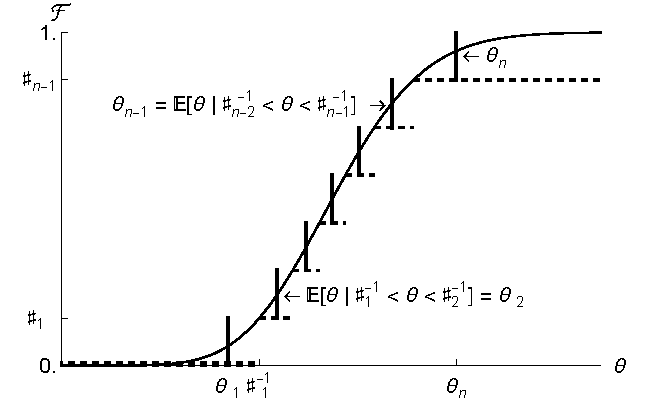
\includegraphics[width=4in]{./Figures/discreteApprox.pdf}

\end{frame}

\begin{frame}[label=DiscretizeEqn]
\frametitle{Trick: Discretize the Risks}

\begin{equation}\begin{gathered}\begin{aligned}
        \vEnd_{t}^{\prime}({a}_{t})  & =  \Discount \Rfree \PermGroFac_{t+1}^{-\CRRA} \left(\frac{1}{n}\right) \sum_{i=1}^{n} \util^{\prime}\left(\cFunc_{t+1}(\RNrm_{t+1} {a}_{t} + \TranShkEmp_{i})\right)
\end{aligned}\end{gathered}\end{equation}

%  \begin{equation}\begin{gathered}\begin{aligned}
        \vFunc_{\EndStgem}({a}_{\stge-1})  & =   \DiscFac \vNormedPermGroFac\left(\frac{1}{n_{\TranShkEmp}}\right)\sum_{i=1}^{n_{\TranShkEmp}}   \frac{\left(\RNrm_{\stge} {a}_{\stge} + \TranShkEmp_{i}\right)^{1-\CRRA}}{1-\CRRA} \label{eq:vDiscrete}
      \end{aligned}\end{gathered}\end{equation}


\pause 
So for any particular $\mRat_{T-1}$ the corresponding $\cNrm_{T-1}$ can be found
using the FOC:
  \begin{equation}\begin{gathered}\begin{aligned}
        \uFunc^{{c}}({c}_{\stge})   & = \vEndStge^{{a}}({m}_{\stge}-{c}_{\stge}).
        \label{eq:upEqbetaOp}
      \end{aligned}\end{gathered}\end{equation}



\end{frame}
\subsection{Interpolate a Consumption Rule}
\begin{frame}
\frametitle{Trick: Interpolate a Consumption Rule}

\begin{enumerate}
\item Define a grid of points $\vec{\mRat}$ (indexed $\mRat[i]$)
\item Use numerical rootfinder to solve 
$\util^{\prime}(\cNrm) = \vEnd^{\prime}_{t}(\mRat[i]-\cNrm)$
\begin{itemize}
\item The $\cNrm$ that solves this becomes $\cNrm[i]$
\end{itemize}
\item Construct interpolating function $\grave{\cFunc}$ by linear interpolation
\begin{itemize}
\item `Connect-the-dots'
\end{itemize}
\end{enumerate}

\end{frame}






\begin{frame}[label=DiscretizeEqn]
\frametitle{Trick: Interpolate a Consumption Rule}

Example: $\vec{\mRat}_{T-1} = \{0.,1.,2.,3.,4.\}$ (solid is `correct' soln)

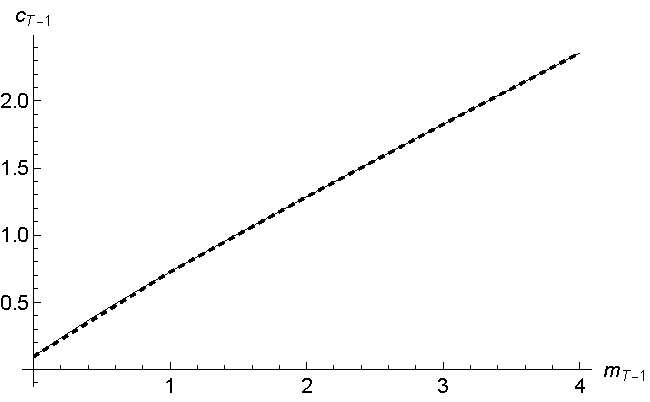
\includegraphics[width=4.0in]{./Figures/PlotcTm1Simple.pdf}

\end{frame}

\begin{frame}[label=vEndtSlow]
\frametitle{Problem: Numerical Rootfinding is {\it Slow}}

Numerical search for values of $\cNrm_{T-1}$ satisfying
$\util^{\prime}(\cNrm) = \vEnd^{\prime}_{t}(\mRat[i]-\cNrm)$ at, say,
6 gridpoints of $\vec{\mRat}_{T-1}$ may require hundreds or even thousands of
evaluations of
\begin{equation}\begin{gathered}\begin{aligned}
        \vEnd^{\prime}_{T-1}(\overbrace{{m}_{T-1}-{\cNrm}_{T-1}}^{\aRat_{T-1}})  & =   \Discount_{T} \PermGroFac_{T}^{1-\CRRA}\left(\frac{1}{n}\right)\sum_{i=1}^{n}   \left( \RNrm_{T} {a}_{T-1} + \TranShkEmp_{i}\right)^{-\CRRA} \notag
\end{aligned}\end{gathered}\end{equation}

\end{frame}




\begin{comment}

\begin{frame}[label=vApprox]
\frametitle{Solution: Approximate $\vEnd$?}

\pause Given $\{\vec{\aRat}_{T-1},\vec{\vEnd}_{T-1}\}$, an approximate function $\grave{\vEnd}_{T-1}$ 
can be constructed by linear interpolation among the points:

\includegraphics[width=4in]{./Figures/PlotOTm1RawVsInt.pdf}

\end{frame}

\begin{frame}
\frametitle{Using $\grave{\vEnd}_{T-1}$ In Optimization}
\begin{equation*}\begin{gathered}\begin{aligned}
  \vFunc_{t}(\mRat_{t})  & = \max_{\cNrm_{t}}~~ \util(\cNrm_{t}) + \grave{\vEnd}_{t}(\mRat_{t}-\cNrm_{t})
\end{aligned}\end{gathered}\end{equation*}
is {\it much} faster,  but result is bad:
\begin{center}
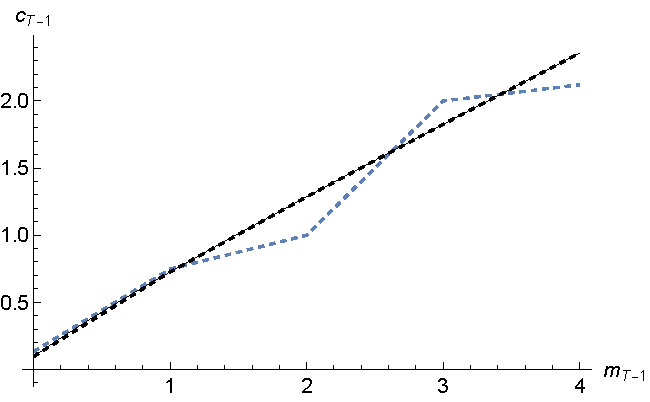
\includegraphics[width=3in]{./Figures/PlotComparecTm1AB}
\end{center}

\end{frame}


\begin{frame}
\frametitle{Approximate $\vEnd_{t}^{\prime}(\aRat)$?}

Better ... but still violates first two principles:
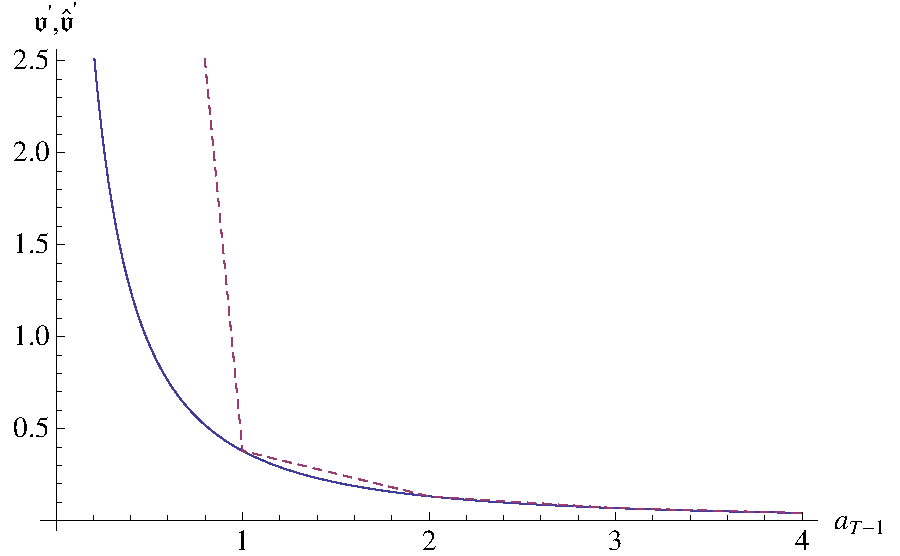
\includegraphics[width=4in]{./Figures/PlotOPRawVSFOC.pdf}

\end{frame}


\end{comment}

\subsection{The Method of Endogenous Gridpoints}
\begin{frame}
\frametitle{Solution: The Method of Endogenous Gridpoints}

\pause 

\begin{itemize}
\item Define vector of {\it end-of-period} asset values $\vec{\aRat}$
\item For each $\aRat[j]$ compute $\vEnd_{t}^{\prime}(\aRat[j])$
\end{itemize}

\pause 

Each of these $\vEnd_{t}^{\prime}[j]$ corresponds to a unique
$\cNrm[j]$ via FOC:
\begin{equation}\begin{gathered}\begin{aligned}
  \cNrm[j]^{-\CRRA}  & = \vEnd_{t}^{\prime}(\aRat[j])
\\ \cNrm[j]  & = \left(\vEnd_{t}^{\prime}(\aRat[j])\right)^{-1/\CRRA}
\end{aligned}\end{gathered}\end{equation}

\pause 

But the DBC says
\begin{equation}\begin{gathered}\begin{aligned}
  \aRat_{t}  & = \mRat_{t} - \cNrm_{t}
\\ \mRat[j]  & = \aRat[j]+\cNrm[j]
\end{aligned}\end{gathered}\end{equation}

\pause 
So computing $\vEnd_{t}^{\prime}$ at a vector of $\vec{\aRat}$ values has produced for us the corresponding $\vec{\cNrm}$ and $\vec{\mRat}$ 
values at virtually no cost!  

\pause 
\medskip 
From these we can interpolate as before to construct $\grave{\cFunc}_{t}(\mRat)$.

\end{frame}


\begin{frame}
\frametitle{Why Directly Approximating $\vFunc_{t}$ is a Bad Idea}

Principles of Approximation

\begin{itemize}
\item Hard to approximate things that approach $\infty$ for relevant $\mRat$
\begin{itemize}
\item Not a prob for Rep Agent models: `relevant' $\mRat$'s are $\approx$ SS
\end{itemize}
\item Hard to approximate things that are highly nonlinear 
%\item Best to approximate things that directly govern behavior
\end{itemize}


\end{frame}


\begin{frame}
\frametitle{Approximate Something That Would Be Linear in PF Case}

\medskip

Perfect Foresight Theory:
\begin{equation}\begin{gathered}\begin{aligned}
  \cFunc_{t}(\mRat)  & = (\mRat+\hEnd_{t})\MPCmin_{t} 
\end{aligned}\end{gathered}\end{equation}
for market resources $\mRat$ and end-of-period human wealth $\hEnd$.


\medskip\medskip
\pause 

This is why it's a good idea to approximate $\cFunc_{t}$ 

\pause \medskip\medskip

Bonus: Easy to debug programs by setting $\sigma^{2} = 0$ and
testing whether numerical solution matches analytical!

\end{frame}

\subsection{Approximate Inverted Functions}
\begin{frame}%[ValFnApprox]
\frametitle{But What if You {\it Need} the Value Function?}

Perfect foresight value function:
  \begin{equation}\begin{gathered}\begin{aligned}
        \bar{\vFunc}_{t}({m}_{t})  & = \uFunc(\bar{\cNrm}_{t})\mathbb{C}_{t}^{T}\label{eq:vFuncPF}
        \\  & = \uFunc(\bar{c}_{t}) \MPCmin_{t}^{-1} % 20190820
        \\  & = \uFunc((\aboveMin \mNrm_{t}+\aboveMin \hEnd_{t})\MPCmin_{t}) \MPCmin_{t}^{-1} % 20190820
        \\  & = \uFunc(\aboveMin \mNrm_{t}+\aboveMin \hEnd_{t})\MPCmin_{t}^{1-\CRRA} \MPCmin_{t}^{-1} % 20190820
        \\  & = \uFunc(\aboveMin \mNrm_{t}+\aboveMin \hEnd_{t})\MPCmin_{t}^{-\CRRA}  % 20190820
      \end{aligned}\end{gathered}\end{equation}
  where the second line uses the fact demonstrated in \cite{BufferStockTheory} that $\mathbb{C}_{t}=\MPC^{-1}_{t}$. % 20190820

  This can be transformed as
  \begin{equation*}\begin{gathered}\begin{aligned}
        \bar{\vInv}_{t}  & \equiv  \left((1-\CRRA)\bar{\vFunc}_{t}\right)^{1/(1-\CRRA)}
        \\  & = \cNrm_{t}(\mathbb{C}_{t}^{T})^{1/(1-\CRRA)}
        \\  & = (\aboveMin \mNrm_{t}+\aboveMin \hEnd_{t})\MPCmin_{t}^{-\CRRA/(1-\CRRA)}   % 20190820
      \end{aligned}\end{gathered}\end{equation*}

which is linear.  

\medskip\medskip
\pause If you need the value function, approximate the {\it inverted} value function to generate $\grave{\vInv}_{t}$ 
and then obtain your approximation from 
\begin{equation}\begin{gathered}\begin{aligned}
  \grave{\vFunc}_{t}  & = \util(\grave{\vInv}_{t})
\end{aligned}\end{gathered}\end{equation}


\end{frame}

\subsection{Derivatives}
\begin{frame}
\frametitle{Approximate Slope Too}

\cite{BufferStockTheory} shows that $\cFunc^{\mRat}_{t}$ exists everywhere.
\medskip

\pause 
Define {\it consumed} function and its derivative as 
\begin{equation}\begin{gathered}\begin{aligned}
  \cEndFunc_{t}(\aRat)  & = (\vEnd^{\prime}_{t}(\aRat))^{-1/\CRRA}
\\ \cEndFunc_{t}^{\aRat}(\aRat)  & = -(1/\CRRA)\left(\vEnd_{t}^{\prime}({a})\right)^{-1-1/\CRRA} \vEnd_{t}^{\prime\prime}(\aRat) 
\end{aligned}\end{gathered}\end{equation}

\pause 
and using chain rule it is easy to show that
\begin{equation}\begin{gathered}\begin{aligned}
 \cFunc^{\mRat}_{t}  & = \cEndFunc^{\aRat}_{t}/(1+\cEndFunc^{\aRat}_{t})
\end{aligned}\end{gathered}\end{equation}

\end{frame}

\begin{frame}
\frametitle{To Implement: Modify Prior Procedures in Two Ways}
\begin{enumerate}
\item Construct $\vec{\cFunc}^{\mRat}_{t}$ along with $\vec{\cFunc}_{t}$ in EGM algorithm
\item Approximate $\cFunc_{t}(m)$ using piecewise Hermite polynomial
\begin{itemize}
\item Exact match to both level and derivative at set of points
\end{itemize}
\end{enumerate}
\end{frame}


\subsection{Improving the $\aRat$ Grid}

\begin{frame}
\frametitle{Problem: $\Alt{\cFunc}$ Below Bottom $\mRat$ Gridpoint and Extrapolation}

Consider what happens as ${a}_{T-1}$ approaches $\underline{a}_{T-1}\equiv-\underline{\TranShkEmp}\RNrm_{T}^{-1}$,
\begin{equation*}\begin{gathered}\begin{aligned}
        \lim_{{\aRat} \downarrow \underline{a}_{T-1}} \vEnd_{T-1}^{\prime}({\aRat}) 
& =         \lim_{{\aRat} \downarrow \underline{a}_{T-1}} \Discount \Rfree \PermGroFac_{T}^{-\CRRA} \left(\frac{1}{n}\right) \sum_{i=1}^{n} \left( {\aRat} \RNrm_{T}+ \TranShkEmp_{i}\right)^{-\CRRA}
\\  & = \infty
\end{aligned}\end{gathered}\end{equation*}

This means our lowest value in $\vec{\aRat}_{T-1}$ should be $> \underline{\aRat}_{T-1}$.  

\medskip
Suppose we construct $\Alt{\cFunc}$ by linear interpolation:
\begin{equation*}\begin{gathered}\begin{aligned}
  \Alt{\cFunc}_{T-1}(\mRat)  & = \Alt{\cFunc}_{T-1}(\vec{\mRat}_{T-1}[1])+\Alt{\cFunc}_{T-1}^{\prime}(\vec{\mRat}_{T-1}[1])({\mRat}-\vec{\mRat}_{T-1}[1]) \label{eq:ExtrapLin}
\end{aligned}\end{gathered}\end{equation*}

True $\cFunc$ is strictly concave 
$\Rightarrow \exists \mRat^{-} > \underline{\mRat}_{T-1}$  for which $\mRat^{-}-\Alt{\cFunc}_{T-1}(\mRat^{-}) < \underline{\aRat}_{T-1}$

\end{frame}

\begin{frame}
\frametitle{Solution: Hard-Code the Bottom Point}

Theory says that
\begin{equation}\begin{gathered}\begin{aligned}
  \lim_{\mRat \downarrow \underline{\mRat}_{T-1}} \cFunc_{T-1}(\mRat)  & = 0
\\ \lim_{\mRat \downarrow \underline{\mRat}_{T-1}} \cFunc_{T-1}^{\mRat}(\mRat)  & = \MPCmax_{T-1}
\end{aligned}\end{gathered}\end{equation}

\medskip 

\begin{enumerate}
\item Redefine $\vec{\aRat}$ {\it relative} to $\uline{\aRat}_{T-1}$
\item Construct corresponding $\vec{\mRat}_{T-1}$ and $\vec{\cNrm}_{T-1}$
\item Prepend $\uline{\mRat}_{T-1}$ to $\vec{\mRat}_{T-1}$
\item Prepend $0.$ to $\vec{\cNrm}_{T-1}$
\item Prepend $\MPCmax_{T-1}$ to $\vec{\MPC}_{T-1}$
\end{enumerate}
then proceed as before.

\end{frame}

\begin{frame}
\frametitle{Trick: Improving the $\aRat$ Grid}
Grid Spacing: Uniform

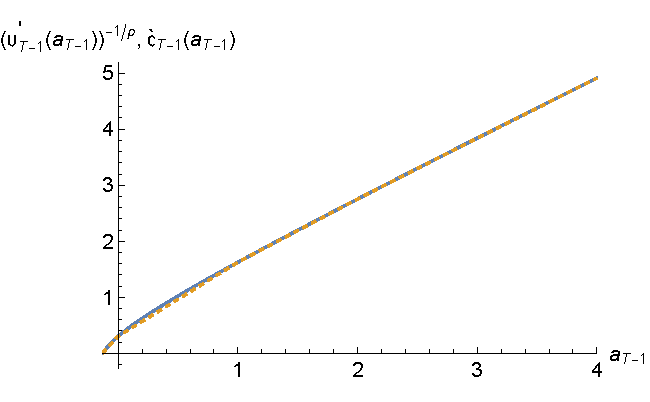
\includegraphics[width=4in]{./Figures/GothVInvVSGothC.pdf}

\end{frame}


\begin{frame}
\frametitle{Trick: Improving the $\aRat$ Grid}
Grid Spacing: Same $\{\uline{\aRat},\bar{\aRat}\}$ But Triple Exponential $e^{e^{e^{...}}}$ Growth

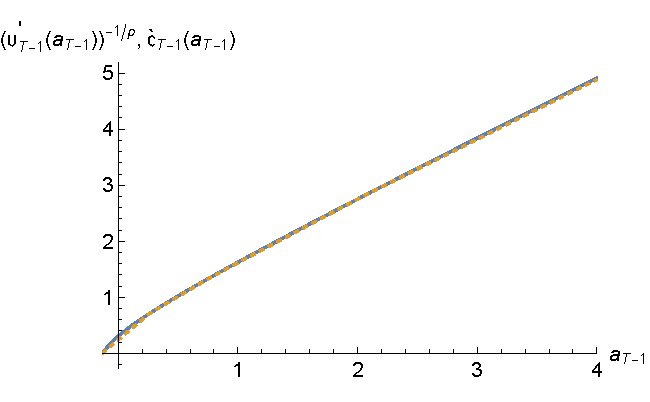
\includegraphics[width=4in]{./Figures/GothVInvVSGothCEEE.pdf}

\end{frame}


\subsection{The Method of Moderation}

\begin{frame}[label=MoM]
\frametitle{The Method of Moderation}

\begin{itemize}
\item Further improves speed and accuracy of solution
\item See my talk at the conference!
\end{itemize}

\end{frame}

\begin{frame}
\frametitle{Imposing `Artificial' Borrowing Constraints}
\begin{eqnarray*}
{\vFunc}_{T-1}({m}_{T-1}) & = & \max_{\cNrm_{T-1}} ~~ \util({c}_{T-1}) + \Ex_{T-1} [\Discount \PermGroFac_{T}^{1-\CRRA}{\vFunc}_{T}({m}_{T})] \label{eq:ConstrArt}
\\ & \mbox{s.t.}&  \nonumber
\\ {a}_{T-1} & = & {m}_{T-1} - {c}_{T-1}
\\ {m}_{T} & = & \RNrm_{T} {a}_{T-1} + \TranShkEmp_{T}
\\ {a}_{T-1} & \geq & 0 .
\end{eqnarray*}


\pause 

Define $\grave{\cFunc}^{*}_{t}$ as soln to unconstrained problem.  Then
  \begin{equation}\begin{gathered}\begin{aligned}
        \grave{\cFunc}_{T-1}({m}_{T-1})  & = \min[{m}_{T-1},\grave{\cFunc}^{\ast}_{T-1}({m}_{T-1})] \label{eq:LiqCons}.
      \end{aligned}\end{gathered}\end{equation}


\end{frame}

\begin{frame}
\frametitle{Imposing `Artificial' Borrowing Constraints}

Point where constraint makes transition from binding to not is
\begin{equation*}\begin{gathered}\begin{aligned}
    \util^{\prime}(\mRat_{T-1}^{\#})  & = \vEnd^{\prime}_{T-1}(0.)
\\  \mRat_{T-1}^{\#}  & = \left(\vEnd^{\prime}_{T-1}(0.)\right)^{-1/\CRRA}
\end{aligned}\end{gathered}\end{equation*}
\pause\medskip

Procedure is very easy:
\begin{itemize}
\item Add $0.$ as first point in $\vec{\aRat}$
\item $\Rightarrow \vec{\mRat}[1] = \mRat_{T-1}^{\#}$
\item Above $\mRat_{T-1}^{\#}$, $\grave{\cFunc}_{T-1}(\mRat)$ obtained as before
\item Below $\mRat_{T-1}^{\#}$, $\grave{\cFunc}_{T-1}(\mRat)=\mRat$
\end{itemize}

\end{frame}

\begin{frame}
\frametitle{Imposing `Artificial' Borrowing Constraints}
\begin{figure}
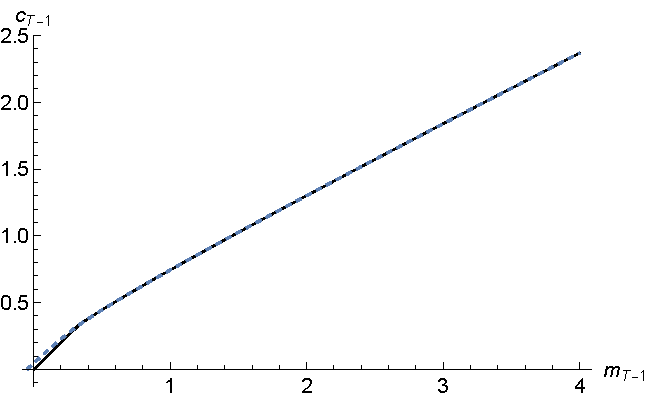
\includegraphics[width=4in]{./Figures/cVScCon.pdf}
        \caption{Constrained (solid) and Unconstrained (dashed) Consumption}
        \label{fig:cVScCon}
\end{figure}

\end{frame}

\begin{frame}%[Recursion]
\frametitle{Recursion: Period $t$ Solution Given Period $t+1$}
\begin{enumerate}
\item Construct 
    \begin{equation}\begin{gathered}\begin{aligned}
          \cFunc_{\overline{t},i}  & = \left(\vEndStge^{{a}}({a}_{t,i})\right)^{-1/\CRRA},
          \\                             & = \left(\DiscFac \Ex_{\BegStge} \left[\Rfree \PermGroFac_{t+1}^{-\CRRA}(\grave{\cFunc}_{t+1}(\RNrm_{t+1} {a}_{t,i} +      {\TranShkEmp}_{t+1}))^{-\CRRA}\right]\right)^{-1/\CRRA}, \label{eq:vEndeq}
          \MPCMatch{\\        \cFunc^{a}_{\overline{t},i}  & = -(1/\CRRA)\left(\vEndStge^{{a}}({a}_{t,i})\right)^{-1-1/\CRRA} \vEndStge^{{a}{a}}(\aNrm_{t,i}),}{}
        \end{aligned}\end{gathered}\end{equation}
  

\item Call the result $\vec{\cNrm}_{t}$ and generate the corresponding $\vec{\mRat}_{t}=\vec{\cNrm}_{t}+\vec{\aRat}_{t}$
\item Interpolate to create $\grave{\cNrm}_{t}(\mRat)$
\end{enumerate}

\end{frame}

\begin{frame}%[Convergence]
\frametitle{Consumption Rules $\grave{\cFunc}_{T-n}$ Converge}

\begin{figure}
        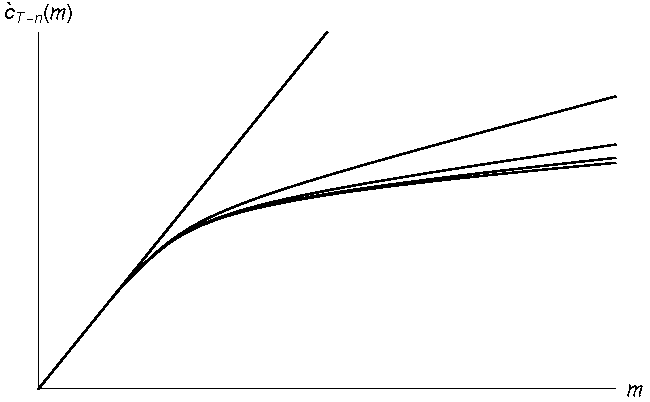
\includegraphics[width=4in]{./Figures/PlotCFuncsConverge.pdf}
        \caption{Converging $\grave{\cFunc}_{T-n}({\mRat})$ Functions for $n=\{1,5,10,15,20\}$}
        \label{fig:PlotCFuncsConverge}
\end{figure}

\end{frame}


\section{Multiple Control Variables}
\begin{frame}
\frametitle{Portfolio Choice}

Now the consumer has a choice between a risky and a safe asset.  \pause The portfolio
return is
  \begin{equation}\begin{gathered}\begin{aligned}
        \Rport_{t+1}  & = \Rfree(1-\varsigma_{t}) + \Risky_{t+1}\varsigma_{t} \label{eq:return1}
        \\               & = \Rfree + (\Risky_{t+1}-\Rfree) \varsigma_{t} %\label{eq:return2}
      \end{aligned}\end{gathered}\end{equation}

\pause so (setting $\PermGroFac=1$) the maximization problem is \pause 
  \begin{equation*}\begin{gathered}\begin{aligned}
        {\vFunc}_{t}({m}_{t})  & = \max_{\{{c}_{t},\varsigma_{t}\}}   ~~ \uFunc({c}_{t}) +  \DiscFac
        \Ex_{t}[{\vFunc}_{t+1}({m}_{t+1})]
        \\      & \text{s.t.} & \nonumber
        \\      \Rport_{t+1}  & = \Rfree + (\Risky_{t+1}-\Rfree) \varsigma_{t}
        \\      {m}_{t+1}  & = ({m}_{t}-{c}_{t})\Rport_{t+1} + \TranShkEmp_{t+1}
        \\  0       \leq & \varsigma_{t}  \leq 1, \label{eq:noshorts}
      \end{aligned}\end{gathered}\end{equation*}


\end{frame}

\begin{frame}
\frametitle{Portfolio Choice}

The FOC with respect to $\cNrm_{t}$ now yields an Euler equation
  \begin{equation}\begin{gathered}\begin{aligned}
        \uFunc^{{c}}({c}_{t})  & = \Ex_{t}[\DiscFac {\Rport}_{t+1} \uFunc^{{c}}({c}_{t+1})]. \label{eq:EulercRiskyR}
      \end{aligned}\end{gathered}\end{equation}

\pause
while the FOC with respect to the portfolio share yields
  \begin{equation}\begin{gathered}\begin{aligned}
        0  & = \Ex_{t}[{\vFunc}_{\MidStepp}^{{m}}({m}_{t+1})(\Risky_{t+1}-\Rfree){a}_{t}] \notag
        \\         & = {a}_{t}\Ex_{t}\left[\uFunc^{{c}}\left(\cFunc_{t+1}({m}_{t+1})\right)(\Risky_{t+1}-\Rfree)\right] \label{eq:FOCw}.
      \end{aligned}\end{gathered}\end{equation}


\end{frame}

\section{The Infinite Horizon}
\subsection{Convergence}
\begin{frame}
\frametitle{Convergence}

When the problem satisfies certain conditions~(\cite{BufferStockTheory}),
it defines a `converged' consumption rule with a `target' ratio $\check{\mRat}$
that satisfies:
\begin{equation}\begin{gathered}\begin{aligned}
  \Ex_{t}[\mRat_{t+1}/\mRat_{t}]  & = 1 \text{~if $\mRat_{t} = \check{\mRat}$}
\end{aligned}\end{gathered}\end{equation}

\pause 

Define the target $\mRat$ implied by the consumption rule $\cFunc_{t}$ as $\check{\mRat}_{t}$.

\medskip\pause
Then a plausible metric for convergence is to define some value $\epsilon$ and to declare
the solution to have converged when
\begin{equation}\begin{gathered}\begin{aligned}
  |\check{\mRat}_{t+1}-\check{\mRat}_{t}|  & < \epsilon
\end{aligned}\end{gathered}\end{equation}

\end{frame}

\subsection{Tricks}
\begin{frame}
\frametitle{Trick: Coarse then Fine $\TranShkEmp$}

\begin{enumerate}
\item Start with coarse grid for $\TranShkEmp$ (say, 3 points)
\item Solve to convergence; call period of convergence $n$
\item Construct finer grid for $\TranShkEmp$ (say, 7 points)
\item Solve for period $T-n-1$ assuming $\Alt{\cFunc}_{T-n}$ 
\item Continue to convergence
\end{enumerate}

\end{frame}

\begin{frame}
\frametitle{Trick: Coarse then Fine $\vec{\aRat}_{T-1}$}

\begin{enumerate}
\item Start with coarse grid for $\vec{\aRat}$ (say, 5 gridpoints)
\item Solve to convergence; call period of convergence $n$
\item Construct finer grid for $\vec{\aRat}$ (say, 20 points)
\item Solve for period $T-n-1$ assuming $\Alt{\cFunc}_{T-n}$ 
\item Continue to convergence
\end{enumerate}

\end{frame}

\section{Structural Estimation}
\subsection{Life Cycle Model}

\begin{frame}
\frametitle{Life Cycle Maximization Problem}
  \begin{equation*}\begin{gathered}\begin{aligned}
        {\vFunc}_{t}({m}_{t})  & = \max_{{c}_{t}}~~~ \uFunc({c}_{t})+\beth\Alive_{t+1}\hat{\DiscFac}_{t+1}
          \Ex_{t}[(\PermShk_{t+1}\PermGroFac_{t+1})^{1-\CRRA}{\vFunc}_{t+1}({m}_{t+1})]   \\
        & \text{s.t.} &   \nonumber \\
        {a}_{t}    & = {m}_{t}-{c}_{t} \nonumber
        \\      {m}_{t+1}  & = {a}_{t}\underbrace{\left(\frac{\Rfree}{\PermShk_{t+1}\PermGroFac_{t+1}}\right)}_{\equiv \RNrm_{t+1}}+ ~\TranShkEmp_{t+1}
      \end{aligned}\end{gathered}\end{equation*}

  \begin{equation*}\begin{gathered}\begin{aligned}
        \Alive _{t}^{t+n} &:\text{probability to }\Alive\text{ive until age $t+n$ given alive at age $t$}
        \\      \hat{\DiscFac}_{t}^{t+n} &:\text{age-varying discount factor between ages $t$ and $t+n$}
        \\     \Psi_{t} &:\text{mean-one shock to permanent income}
        \\     \beth &:\text{time-invariant `pure' discount factor}
      \end{aligned}\end{gathered}\end{equation*}

\end{frame}

\begin{frame}
\frametitle{Details follow~\cite{cagettiWprofiles}}
\begin{itemize}
\item Parameterization of Uncertainty
\item Probability of Death
\item Demographic Adjustments to $\Discount$
\end{itemize}
\end{frame}

\begin{frame}
\frametitle{Empirical Wealth Profiles}
\begin{figure}
    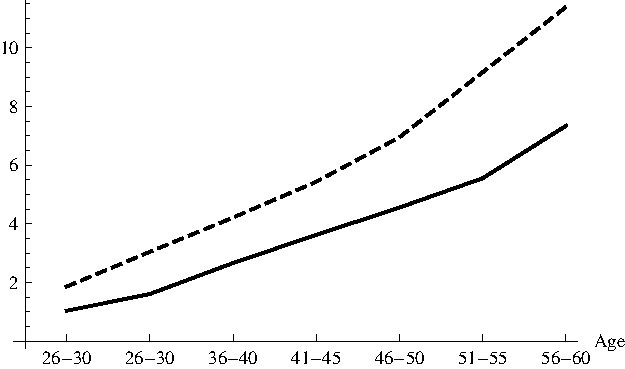
\includegraphics[width=3.5in]{./Figures/PlotMeanMedianSCFcollegeGrads.pdf}
    \caption{$\mRat$ from SCF (means (dashed) and medians (solid))}
    \label{fig:MeanMedianSCF}
\end{figure}
\end{frame}

\begin{frame}
\frametitle{Simulated Moments}

Given a set of parameter values $\{\CRRA,\beth\}$:
\begin{itemize}
\item Start at age 25 with empirical $\mRat$ data
\item Draw shocks using calibrated $\sigma^{2}_{\PermShk}$,$\sigma^{2}_{\TranShkEmp}$
\item Consume according to solved $\cFunc_{t}$
\end{itemize}
\pause 
$\Rightarrow \mRat$ distribution by age
\end{frame}

\begin{frame}
\frametitle{Choose What to Simulate}
  \begin{equation}\begin{gathered}\begin{aligned}
        \lefteqn{    \texttt{GapEmpiricalSimulatedMedians$[\CRRA,\beth]$:=}}    \nonumber \\
        &[&\texttt{ConstructcFuncLife$[\CRRA,\beth]$;}\nonumber\\
        &\texttt{Simulate;}\nonumber\\
        &\sum\limits_{i}^{N}\weight _{i}\left|\varsigma_{i}^{\tau }-\mathbf{s}^{\tau}(\xi )\right| \nonumber\\
        &];&\nonumber
      \end{aligned}\end{gathered}\end{equation}

\end{frame}

\begin{frame}
\frametitle{Calculate Match Between Theory and Data}
\begin{equation}\begin{gathered}\begin{aligned}
\xi  & = \{\CRRA,\beth\}
\end{aligned}\end{gathered}\end{equation}
solve
  \begin{equation}
    \min_{\xi}\sum\limits_{i}^{N}\weight _{i}\left|\varsigma_{i}^{\tau }-\mathbf{s}^{\tau}(\xi )\right|\label{eq:StructEstim}
  \end{equation}


\end{frame}
\begin{frame}
\frametitle{Bootstrap Standard Errors (\cite{horowitzBootstrap})}

Yields estimates of 
  \begin{table}[h]
    \caption{Estimation Results}\label{tab:EstResults}
    \center
    \begin{tabular}{cc}
      \hline
      $\CRRA $ & ${\beth}$\\
      \hline
      $3.69$ & $0.88$\\
      $(0.047)$ & $(0.002)$\\
      \hline
    \end{tabular}
  \end{table}


\end{frame}

\begin{frame}
\frametitle{Contour Plot}
\begin{figure}
     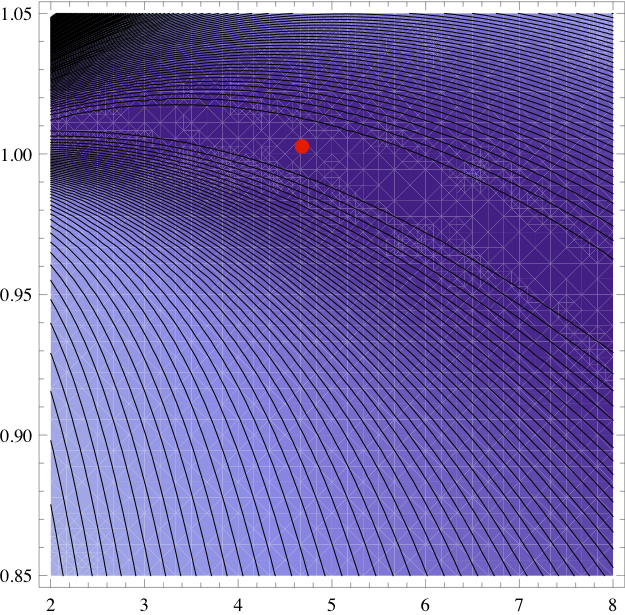
\includegraphics[width=2.5in]{./Figures/PlotContourMedianStrEst.pdf}
    \caption{Point Estimate and Height of Minimized Function}
    \label{fig:PlotContourMedianStrEst}
\end{figure}

\end{frame}

\beamerdefaultoverlayspecification{<*>}

\begin{frame}[allowframebreaks]
\frametitle{\textbf{References}}
\tiny
\input handoutBibMake
\end{frame}


\end{document}
